%
% fig-koordinaten.tex
%
% (c) 2024 Prof Dr Andreas Müller
%
\begin{figure}
\centering
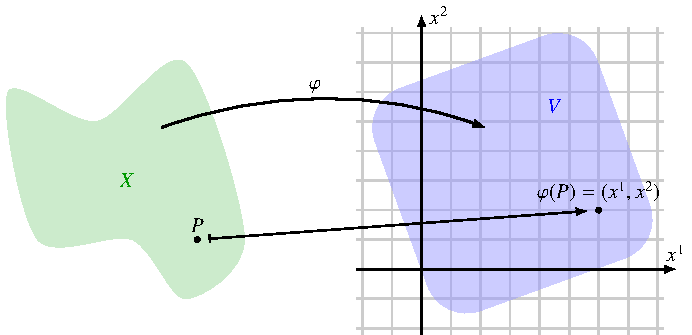
\includegraphics{chapters/020-koordinaten/images/koordinaten.pdf}
\caption{Ein Koordinatensystem auf der Punktmenge $X$ ist eine Abbildung 
$\varphi$ in den Koordinatenraum $V$, der eine Teilmenge von
$\mathbb{R}^n$ ist.
\label{buch:koordinaten:koordinaten:fig:koordinaten}}
\end{figure}
